\chapter{WagonSim}
\label{ch:wagonSim}
% ##################################################################################################################

\hfill \textbf{Author:} Michael Balmer

\begin{center} 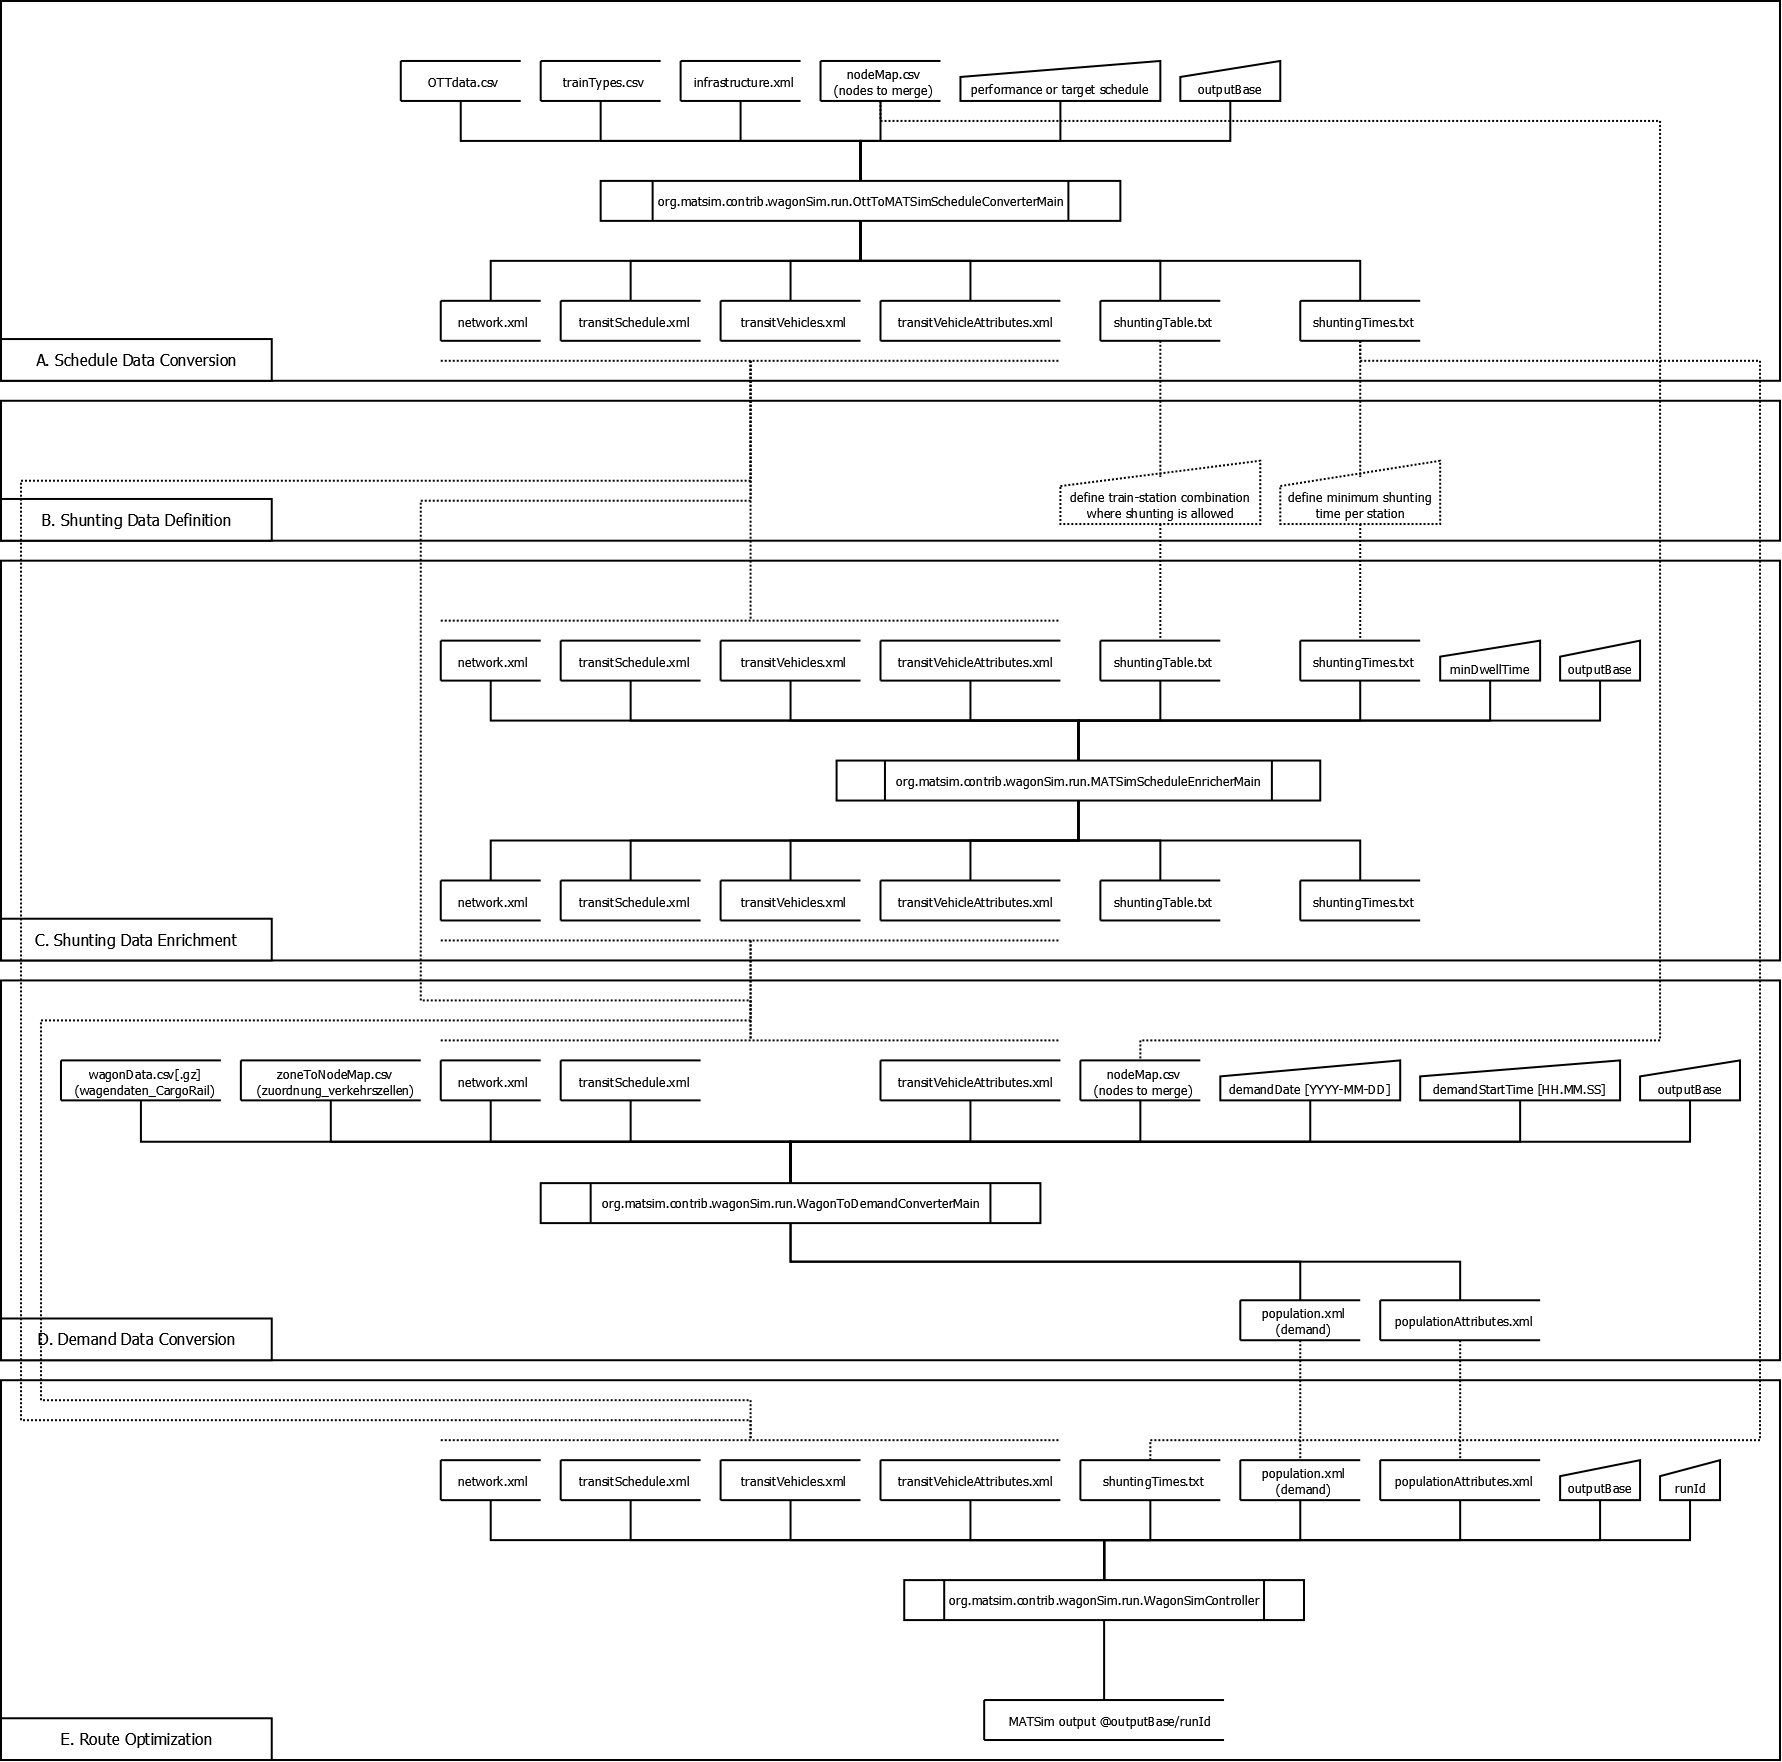
\includegraphics[width=0.25\textwidth, angle=0]{extending/figures/wagonsim/wagonSimProcessChain.png} \end{center}

\editdone{This text has undergone the professional edit. Please no grammatical changes anymore! They are most-probably wrong.}


\createStandardInformationBasic%
{\entryStd{wagonSim}}%
{\invokeStd{wagonSim}{\lstinline|RunWagonSim| class}}%
{No standard configuration.}
{-}

% ##################################################################################################################
%\ah{taken from \url{http://www.matsim.org/extensions/wagonSim} and slightly adapted}
The wagonSim \gls{contribution} allows use of \gls{matsim}'s route-optimization process to find optimal paths for rail-based freight wagons in a given rail-based freight infrastructure.

The network links, here, define the rails, nodes define train stations and schedule transit stops define train station stopping points. 
Freight locomotives are driven by a strictly fixed schedule, where each locomotive is given as a single transit line with a single transit route and a single departure. 
Freight wagons correspond to agents with a given origin and destination (single trip agents). 
Routing takes various constraints into account, \ie a minimum shunting time while switching locomotives and maximum freight train weight and length; it also differentiates between locomotive stops for shunting and stops  only for waiting (without shunting possibility).

WagonSim \gls{contribution} is based on specialized input data. 
The first step converts input data into \gls{matsim} formats (scenario data). In a second step, it allows one to manually adapt the scenario for different parametrization of train stops, shunting stations, minimum shunting times and dwell times of trains at stops. 
The third step sets up route optimization configuration and runs the \gls{matsim} optimization cycle.

As shown at \url{http://www.matsim.org/docs/extensions/wagonSim} and in Figure~\ref{fig:wagonSimProcessChain}, data conversion and WagonSim execution is composed of five stages, described in more detail at above referenced url:
%
\begin{enumerate}[label=\emph{\Alph*})]
\item Schedule data conversion
\item Shunting data definition
\item Shunting data enrichment
\item Demand data conversion
\item Route optimization
\end{enumerate}
%
WagonSim \gls{contribution} has been applied to \gls{eth}, \gls{ivt} Transport Systems group projects.

\createfigure%
{WagonSim process chain}%
{WagonSim process chain}%
{\label{fig:wagonSimProcessChain}}%
{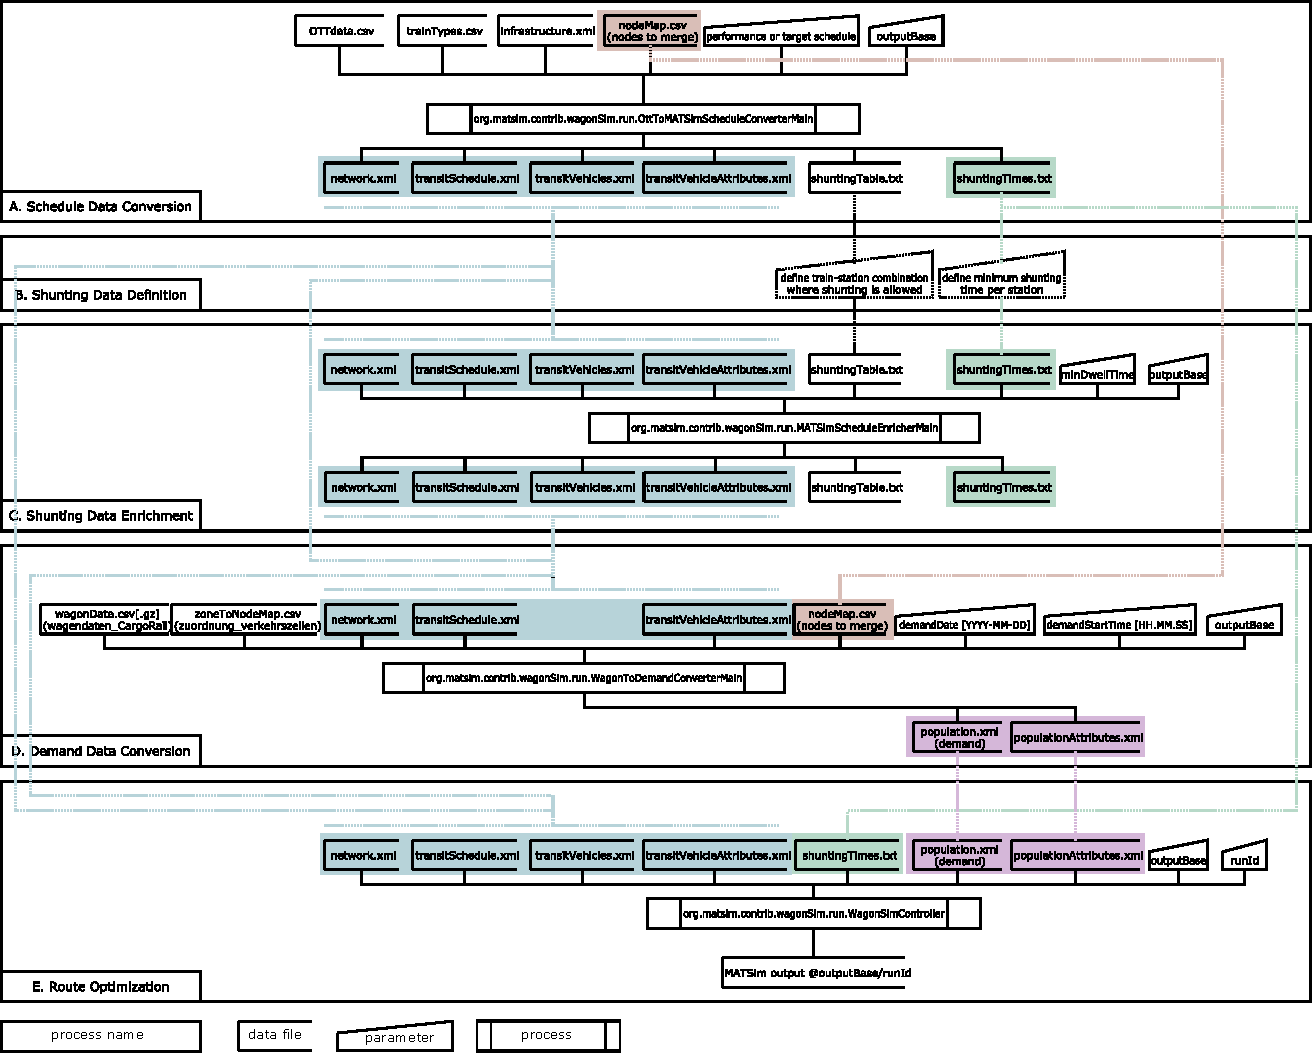
\includegraphics[width=1.22\textwidth,angle=90]{extending/figures/wagonsim/processChainsCompact}}%
{}

% ##################################################################################################################
